\documentclass[epsfig,10pt,fullpage]{article}

\newcommand{\LabNum}{2}
\newcommand{\CommonDocsPath}{../../common/docs}
\addtolength{\textwidth}{1.5in}
\addtolength{\oddsidemargin}{-0.75in}
\addtolength{\topmargin}{-0.75in}
\addtolength{\textheight}{1.5in}
\addtolength{\evensidemargin}{0.75in}
\setlength\parindent{0pt}
\raggedbottom

\usepackage{ae,aecompl}
\usepackage{epsfig,float,times}
\usepackage[hypcap]{caption}
\usepackage[pdftex, colorlinks]{hyperref}
\usepackage{graphicx}
\usepackage[usenames, dvipsnames]{color}
\usepackage{rotating}
\usepackage{tikz}
\usetikzlibrary{automata,positioning}
\usepackage{placeins}

\widowpenalty 10000
\clubpenalty 10000

\newcommand{\red}[1]{{\color{red}\sf{#1}}}
\newcommand{\green}[1]{{\color{green}\sf{#1}}}
\newcommand{\blue}[1]{{\color{blue}\sf{#1}}}
\definecolor{PineGreen}{rgb}{0.0, 0.47, 0.44}
\definecolor{ForestGreen}{rgb}{0.13, 0.55, 0.13}
\definecolor{Brown}{rgb}{0.59, 0.29, 0.0}

\newcommand{\UPDatePublished}{Oct 2021}
\newcommand{\versnum}{21.1} %version number quartus/AMP
\newcommand{\quartusname}{Quartus\textsuperscript{\textregistered} Prime}	
\newcommand{\UPTextBar}{For \quartusname{} \versnum{}}
\newcommand{\thisyear}{2021 } %for copyright
\newcommand{\company}{FPGAcademy.org}
\newcommand{\longteamname}{FPGAcademy.org}
\newcommand{\teamname}{FPGAcademy}
\newcommand{\website}{FPGAcademy.org}

\newcommand{\productAcronym}{AMP}
\newcommand{\productNameShort}{Monitor Program}

\newcommand{\productNameMedTM}{A Monitor Program}
\newcommand{\productNameMed}{A Monitor Program}

%\newcommand{\headerLogoFilePath}[1]{#1/FPGAcademy.png}

% listings is a package that supports encapsulating source code in LaTeX conveniently
\usepackage{listings}

\def\expandparam\lstinputlisting[#1]#2{\edef\tmp{\noexpand\lstinputlisting[#1]{#2}}\tmp}

%%%%%%%%%%%%%%%%%%%% Source Code Formatting %%%%%%%%%%%%%%%%%%%%
\definecolor{globalCommentColour}{rgb}{0.588,0.588,0.588}

%%%%%%%%%%%%%%%%%%%%%%%%%%%%%%%%%%%%%%%%%%%%%%%%%%%%
% Defining language style
% NiosII ASM
\lstdefinelanguage[NiosII]{Assembler} {
  morekeywords={add, addi, and, andhi, andi, beq, bge, bgeu, bgt, bgtu, ble,  bleu, blt, bltu, bne, br, break,% 
  bret, call, callr, cmpeq, cmpeqi, cmpge, cmpgei, cmpgeu, cmpgeui, cmpgt, cmpgti, cmpgtu, cmpgtui, cmple,%
  cmplei, cmpleu, cmpleui, cmplt, cmplti, cmpltu, cmpltui, cmpne, cmpnei, custom, div, divu, eret, flushd,%
  flushda, flushi, flushp, initd, initda, initi, jmp, jmpi, ldb, ldbio, ldbu, ldbuio, ldh, ldhio, ldhu, ldhuio,%
  ldw, ldwio, mov, movhi, movi, movia, movui, mul, muli, mulxss, mulxsu, mulxuu, nextpc, nop, nor, or, orhi, ori,%
  rdctl, rdprs, ret, rol, roli, ror, sll, slli, sra, srai, srl, srli, stb, stbio, sth, sthio, stw, stwio,%
  sub, subi, sync, trap, wrctl, wrtcl, wrprs, xor, xori, xorhi, xori},% 	
  morekeywords=[2]{.abort, .ABORT, .align, .app-file, .ascii, .asciz, .balign, .byte, .comm, .data, .def,%
  .desc, .dim, .double, .eject, .else, .end, .endef, .endif, .equ, .equiv, .err, .extern, .file, .fill, .float,%
  .global, .globl, .hword, .ident, .if, .include, .int, .irp, .irpc, .lcomm, .lflags, .line, .linkonce, .ln,%
  .list, .long, .macro, .mri, .nolist, .octa, .org, .p2align, .psize, .quad, .rept, .sbttl, .scl, .section,%
  .set, .short, .single, .size, .sleb128, .skip, .space, .stadb, .stabn, .stabs, .string, .symver, .tag,%
  .text, .title, .type, .val, .uleb128, .word},% 	
  morekeywords=[3]{et, bt, gp, sp, fp, ea, sstatus, ra, pc, status, estatus, bstatus, ienable, ipending, cpuid,%
  exception, pteaddr, tlbacc, tlbmisc, eccinj, badaddr, config, mpubase, mpuacc},% 	
  sensitive=t,%
  alsoletter=.,%
  morestring=[b]",%
  morecomment=[s]{/*}{*/},%
  morecomment=[l]\#,%
}[keywords,comments,strings]
   
%% NOTE: morekeywords=[2] are GNU directives.
   
\definecolor{niosInstructionColour}{rgb}{0.000,0.608,0.000}
\definecolor{niosDirectiveColour}{rgb}{0.000,0.000,0.902}
\definecolor{niosSpecialRegColour}{rgb}{0.000,0.000,0.000}
\definecolor{niosStringColour}{rgb}{0.808,0.482,0.000}
   
%% NOTE: To make bold use: =\bfseries\color{<colour>}
\lstdefinestyle{defaultNiosStyle} {
  language=[NiosII]{Assembler},
  stringstyle=\color{niosStringColour},
  keywordstyle=\color{niosInstructionColour},
  keywordstyle=[2]\color{niosDirectiveColour},
  keywordstyle=[3]\itshape\color{niosSpecialRegColour}
}
%%%%%%%%%%%%%%%%%%%%%%%%%%%%%%%%%%%%%%%%%%%%%%%%%%%%

%%%%%%%%%%%%%%%%%%%%%%%%%%%%%%%%%%%%%%%%%%%%%%%%%%%%
% Defining language style
% ArmA9 ASM
\lstdefinelanguage[ArmA9]{Assembler} {
  morekeywords={ADC, ADD, ADDS, AND, ANDS, B, BAL, BEQ, BGE, BGT, BL, BLT, BIC, BKPT, BLX, BNE, BX, CDP, CLZ, CMN, CMP, EOR,%
  EORS, LDC, LDM, LDR, LDRB, LDRBT, LDRH, LDRSB, LDRSH, LDRT, LSL, MCR, MLA, MOV, MOVW, MOVT, MRC, MRS, MSR, MUL, MVN, ORR, PLD,%
  ROR, RSB, RSC, SBC, SMLAL, SMULL, STC, STM, STR, STRB, STRBT, STRH, STRT, SUB, SUBS, SWI, SWP, SWPB, TEQ, UMLAL,
  PUSH, POP, MOVS, RORS, LSR},%
  morekeywords=[2]{.abort, .ABORT, .align, .app-file, .ascii, .asciz, .balign, .byte, .comm, .data, .def,%
  .desc, .dim, .double, .eject, .else, .end, .endef, .endif, .equ, .equiv, .err, .extern, .file, .fill, .float,%
  .global, .globl, .hword, .ident, .if, .include, .int, .irp, .irpc, .lcomm, .lflags, .line, .linkonce, .ln,%
  .list, .long, .macro, .mri, .nolist, .octa, .org, .p2align, .psize, .quad, .rept, .sbttl, .scl, .section,%
  .set, .short, .single, .size, .sleb128, .skip, .space, .stadb, .stabn, .stabs, .string, .symver, .tag,%
  .text, .title, .type, .val, .vectors, .uleb128, .word},%
  morekeywords=[3]{SP, PC, MIDR, CTR, TCMTR, TLBTR, MPIDR, ID_PFR0, ID_PFR1, ID_DFR0, ID_MMFR0, ID_MMFR1, ID_MMFR2,%
  ID_MMFR3, ID_ISAR0, ID_ISAR1, ID_ISAR2, ID_ISAR3, ID_ISAR4, CCSIDR, CLIDR, AIDR, CSSELR, TTBR0, TTRB1, TTBR2, DACR,%
  DFSR, IFSR, ADFSR, AIFSR, DFAAR, IFAR, ICIALLUIS, BPIALLIS, PAR, ICIALLU, ICIMVAU, BPIALL, DCIMVAC, DCISW, V2PCWPR,%
  DCCVAC, DCCSW, DDIMVAC, DCISW, TLBALLIS, TLBIMVAIS, TLBIASIDIS, TLBIMVAAIS, TLBIALL, TLBIMVA, TLBIASID, TLBIMVAA,%
  PMCR, PMCNTENSET, PMCNTENCLR, PMOVSR, PMSWINC, PMSELR, PMXEVTYPER, PMXEVCNTR, PMUSERENR, PMINTENSET, PMINTENCLR,%
  PRRR, NRRR, PLEIDR, PLEASR, PLEFSR, PLEUAR, PLEPCR, VBAR, MVBAR, ISR, FCSEIDR, CONTEXTIDR, TPIDRURW, TPIDRURO, TPIDRPRW},%
  sensitive=f,%
  alsoletter=.,%
  morestring=[b]",%
  morecomment=[s]{/*}{*/},%
  morecomment=[l]{//},%
}[keywords,comments,strings]
   
%% NOTE: morekeywords=[2] are GNU directives.
   
\definecolor{armInstructionColour}{rgb}{0.000,0.608,0.000}
\definecolor{armDirectiveColour}{rgb}{0.000,0.000,0.902}
\definecolor{armSpecialRegColour}{rgb}{0.000,0.000,0.000}
\definecolor{armStringColour}{rgb}{0.808,0.482,0.000}
   
\lstdefinestyle{defaultArmStyle} {
  language=[ArmA9]{Assembler},
  stringstyle=\color{armStringColour},
  keywordstyle=\color{armInstructionColour},
  keywordstyle=[2]\color{armDirectiveColour},
  keywordstyle=[3]\itshape\color{armSpecialRegColour}
}
%%%%%%%%%%%%%%%%%%%%%%%%%%%%%%%%%%%%%%%%%%%%%%%%%%%%

%%%%%%%%%%%%%%%%%%%%%%%%%%%%%%%%%%%%%%%%%%%%%%%%%%%%
% Defining language style
% FPGAcademy ASM
\lstdefinelanguage{ASM}{
  morekeywords = [1]{mv, mvt, mvne, mvcc, add, sub, st, ld, and, b, bne, beq, bcc, bcs},
  morekeywords = [2]{word, define},
  keywordstyle = [1]\color{ForestGreen},
  keywordstyle = [2]\color{blue},
  sensitive = true,
  morecomment = [l]{//},
}

\lstset{
  language = ASM,
  basicstyle=\small\color{black}\ttfamily,
  commentstyle=\small\color{Brown}\itshape\ttfamily,
  showstringspaces=false,
  frame=none, %lines % boxed listings
  breaklines=true,
  breakatwhitespace=true,
  tabsize=3
}
%%%%%%%%%%%%%%%%%%%%%%%%%%%%%%%%%%%%%%%%%%%%%%%%%%%%

%%%%%%%%%%%%%%%%%%%%%%%%%%%%%%%%%%%%%%%%%%%%%%%%%%%%
% Defining language style
% Java
\definecolor{javaStringColour}{rgb}{0.808,0.482,0}
%%%%%%%%%%%%%%%%%%%%%%%%%%%%%%%%%%%%%%%%%%%%%%%%%%%%

%%%%%%%%%%%%%%%%%%%%%%%%%%%%%%%%%%%%%%%%%%%%%%%%%%%%
% Defining language style
% C
\definecolor{CStringColour}{rgb}{0.808,0.482,0}

\lstset{
  language = C,
  basicstyle=\small\color{black}\ttfamily, 
  commentstyle=\small\color{PineGreen}\itshape\ttfamily,
  keywordstyle=\small\color{blue}\bfseries\ttfamily,
  showstringspaces=false,
  frame=none, %lines % boxed listings
  breaklines=true,
  breakatwhitespace=true,
  tabsize=3
}
%%%%%%%%%%%%%%%%%%%%%%%%%%%%%%%%%%%%%%%%%%%%%%%%%%%%

%%%%%%%%%%%%%%%%%%%%%%%%%%%%%%%%%%%%%%%%%%%%%%%%%%%%
% Defining language style
% Verilog
\definecolor{verilogCommentColour}{rgb}{0.000,0.502,0.000}

\lstdefinestyle{defaultVerilogStyle} {
  language={Verilog},
  keywordstyle=\color{blue},
  commentstyle=\color{verilogCommentColour}
}
%%%%%%%%%%%%%%%%%%%%%%%%%%%%%%%%%%%%%%%%%%%%%%%%%%%%

%%%%%%%%%%%%%%%%%%%%%%%%%%%%%%%%%%%%%%%%%%%%%%%%%%%%
% Defining language style
% VHDL
\lstdefinestyle{defaultVHDLStyle} {
  language={VHDL},
  keywordstyle=\color{blue},
  commentstyle=\color{verilogCommentColour}
}
%%%%%%%%%%%%%%%%%%%%%%%%%%%%%%%%%%%%%%%%%%%%%%%%%%%%

%%%%%%%%%%%%%%%%%%%%%%%%%%%%%%%%%%%%%%%%%%%%%%%%%%%%
% Defining language style
% LaTeX
\lstdefinelanguage[LocalLaTeX]{TeX}[LaTeX]{TeX}{moretexcs={bf, it, sf, lstset},}

\lstdefinestyle{defaultLocalLatexStyle} {
  language=[LocalLatex]{TeX},
  keywordstyle=\color{blue}\bfseries,
  keywordstyle=[2]\color{blue},
  keywordstyle=[3]\color{blue}\bfseries
}
%%%%%%%%%%%%%%%%%%%%%%%%%%%%%%%%%%%%%%%%%%%%%%%%%%%%

%%%%%%%%%%%%%%%%%%%%%%%%%%%%%%%%%%%%%%%%%%%%%%%%%%%%
% Defining language style
% Default
\lstset{
  basicstyle=\small\color{black}\ttfamily,
  commentstyle=\small\color{globalCommentColour}\itshape\ttfamily,
  keywordstyle=\small\color{blue}\bfseries\ttfamily,
  showstringspaces=false,
  frame=none, %lines % boxed listings
  breaklines=true,
  breakatwhitespace=true,
  tabsize=3
}
%%%%%%%%%%%%%%%%%%%%%%%%%%%%%%%%%%%%%%%%%%%%%%%%%%%%


\hypersetup{
  pdftitle={OPAE Lab Exercise \LabNum},
  linkcolor=blue,
  hyperindex=true,
  pdfauthor={FPGAcademy.org},
  pdfkeywords={FPGAcademy.org, FPGAcademy, Lab, Exercise, OPAE},
  bookmarks,
  bookmarksopen=false,
  filecolor=blue,
  pdfstartview={FitH},
  urlcolor=blue,
  plainpages=false,
  pdfpagelabels=true,
  linkbordercolor={1 1 1} %no color for link border
}



\begin{document}

\centerline{\huge OPAE}
~\\
\centerline{\huge Laboratory Exercise \LabNum}
~\\
\centerline{\large Direct Memory Access (DMA)}
~\\

\noindent
The exercise is organized into the following stages:
\begin{enumerate}
    \item Design a hardware component that will perform transformation on an image stored in local memory.
    \item Augment the hardware component described above to create a DMA AFU that can read a source image from the host and write the result image back to the host.
    \item Design software application that utilize the AFU.
\end{enumerate}


\section*{Part I}

% MPF:\\
% CCI-P to CCI-P bridge\\
% maintain the interface and add new semantics\\
% instantiate on top of CCI-P interface to simplify access to CCI-P\\
% Read order buffer: Reorder buffer to sort read responses and return them in request order\\
% CCI-P to Avalon-MM Adaptor\\
Figure \ref{fig:dmaAFU} provides a high-level diagram of a DMA AFU. It communicates with the FPGA Inteface Unit(FIU) with the \emph{Core Cache Interface} protocol (CCI-P). The MMIO Decoder Logic then separates Memory-Mapped IO(MMIO) and the DMA read and write channels. We will use MMIO for control signals and the DMA channels for transfering data between the processor and the AFU, which is discussed in Part II.\\

\begin{figure}[h]
    \centering
    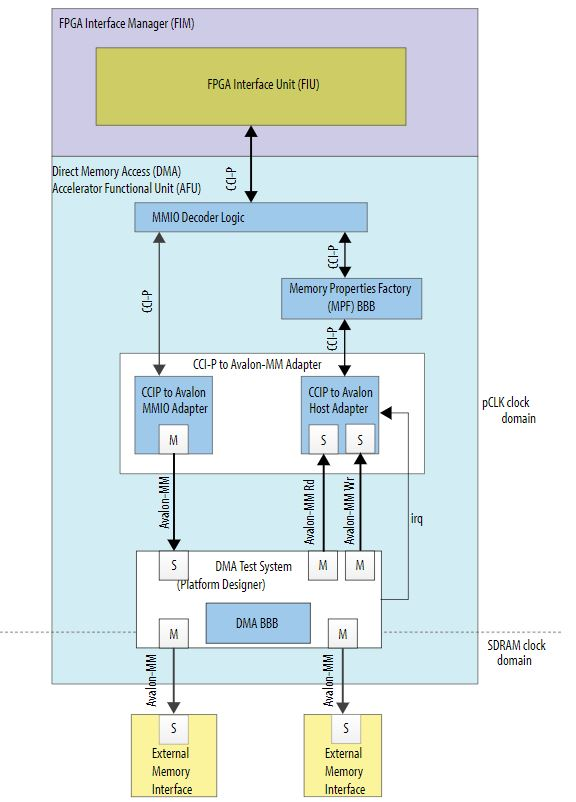
\includegraphics[width=0.5\textwidth]{figures/DMAAFU.JPG}
    \caption{A block diagram of the DMA AFU}
    \label{fig:dmaAFU}
\end{figure}

\newpage
\noindent
In this part of the exercise we will design only the image transformation module of the AFU.  The image transformation module receives a start command from its input port {\it ctrl} along with some information about the transformation to be performed from the input port {\it ctrl\_data}. After receiving the command, the module will create a new image by reading in pixels of the original image and writing the pixels to the corresponding locations in a new pixel array. \\
\\
To align with the signals in other components in the DMA system (in Part II), \emph{ctrl} is 1-bit and \emph{ctrl\_data} is 64-bit. We will use the highest 4 bytes of \emph{ctrl\_data} to specify the number of pixels in the image, the next 2 bytes for the number of pixels in each row and the lowest byte for the type of transformation: 0 for no transformation, 1 for rotate by $180^\circ$ and 2 for horizontally flip. There is another 1-bit input \emph{ctrl\_address} specifying the address of the register to load \emph{ctrl\_data}.  We will take \emph{ctrl\_data} as valid when \emph{ctrl} is 1 AND \emph{ctrl\_address} is 0. \\
\\
The module accesses local memory through a memory interface and it has a parameter {\it n} that specifies the width of the data it read/write from memory. The interface consists of four output ports 48-bit {\it address}, n-bit {\it writedata}, 1-bit {\it read} and {\it write}, and three input ports n-bit {\it readdata}, 1-bit {\it readdatavalid} and 1-bit {\it waitrequest}. The module sends a read/write command out through the interface by setting {\it read} or {\it write} high, and {\it address} to the corresponding location to access.  In response to a {\it read} request, {\it readdata} will be set to the data at {\it address} in memory and {\it readdatavalid} will be set to 1 when {\it readdata} is valid. There is no response for a {\it write} request. The {\it waitrequest} input will be set to 1 when the memory component is unable to process read/write requests. If the module is sending a read or write request when {\it waitrequest} is 1, it needs to maintain the signals until {\it waitrequest} becomes 0.\\
\\
In addition to the signals, the module includes two registers {\it pixel\_counter} and {\it transform\_done}. The {\it pixel\_counter} register keeps track of the number of pixels already processed. The {\it transform\_done} records the status of an image transformation. It should be set to 0 when a new command arrives and set to 1 when a transformation finishes ({\it pixel\_counter}=total number of pixels). The host computer will read the value of {\it transfer\_done} to determine if the AFU completes the image transformation. An enum called transform\_state is used for the FSM state.\\

\begin{figure}[h]
\begin{center}
    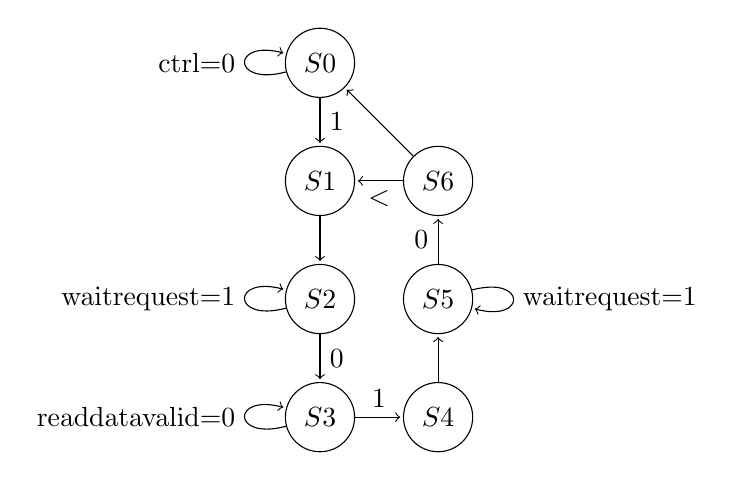
\begin{tikzpicture}[shorten >=1pt,node distance=1.5cm,on grid,auto] 
   \node[state] (S0)   {$S0$}; 
   \node[state] (S1) [below=of S0] {$S1$}; 
   \node[state] (S2) [below=of S1] {$S2$};
   \node[state] (S3) [below=of S2] {$S3$};
   \node[state] (S4) [right=of S3] {$S4$};
   \node[state] (S5) [above=of S4] {$S5$};
   \node[state] (S6) [above=of S5] {$S6$};
    \path[->] 
    (S0) edge  node {1} (S1)
    (S0) edge [loop left] node {ctrl=0} ()
    (S1) edge  node {} (S2)
    (S2) edge [loop left] node {waitrequest=1} ()
    (S2) edge node {0} (S3)
    (S3) edge node {1} (S4)
    (S3) edge [loop left] node {readdatavalid=0} ()
    (S4) edge node {} (S5)
    (S5) edge [loop right] node {waitrequest=1} ()
    (S5) edge node {0} (S6)
    (S6) edge node {} (S0)
    (S6) edge node {$<$} (S1);
\end{tikzpicture}
\end{center}
\caption{A finite state machine.}
\label{fig:FSM}
\end{figure}

\noindent
We can control the process of image transformation using a finite state machine (FSM) controller as in Figure \ref{fig:FSM}. The FSM starts in \textbf{idle} state (S0). After receiving the control signals ($ctrl=1$), it moves to \textbf{read} state (S1) to set \emph{read} and \emph{address} signals. On the next positive clock edge, the FSM transitions to \textbf{read\_req} state (S2) where \emph{read}=1. If \emph{waitrequest} signal is 1, the FSM remains in the \textbf{read\_req} state, otherwise, it changes to \textbf{wait} state (S3), where read is set to 0 again. The FSM stays in the \textbf{wait} state as long as \emph{readdatavalid} is 0. After getting the valid pixels, it moves to \textbf{write} state (S4) to set \emph{write}, \emph{writedata} and \emph{address} signals. Similar to reading from memory, it then transitions to \textbf{write\_req} state (S5) on the next active clock edge. When writing completes, it goes to \textbf{count} state (S6) to increase \emph{pixel\_counter}, and set write to 0 again. The FSM returns to \textbf{read} state if the number of pixels processed is smaller than the total number of pixels in the image, otherwise, it returns to \textbf{idle} state.\\
\\
Perform the following steps to complete the design of the image transformation module with Verilog code:

\lstset{language=Verilog,morekeywords={logic,always_ff},numbers=none,escapechar=|}
\begin{figure}[h]
\begin{center}
\begin{minipage}[h]{15 cm}
\begin{lstlisting}[name=code]
module image_transform(clk, reset, ctrl, ctrl_data, ctrl_address, readdata, readdatavalid, waitrequest, address, read, write, writedata);

    parameter NUM_BYTES = 2, n = 16;
    input clk, reset, ctrl, ctrl_address;
    input [63:0] ctrl_data;
    input [n-1:0] readdata;
    input readdatavalid, waitrequest;
    output logic [47:0] address;
    output logic read, write;
    output logic [n-1:0] writedata;

    logic transform_done;
    logic [31:0] pixel_counter;
    logic [15:0] pixel_per_row;
    logic [47:0] src_address, dst_address;
    logic [ 7:0] transform_type;
    |$\ldots$| declare other signals

    always @(posedge clk) begin
        if(reset) begin
            src_address <= '0; dst_address <= '0; 
            transform_type <= '0;
        end
        else if(ctrl && ctrl_address == 0) begin    
            // read instructions
            src_address <= '0;
            dst_address[31:0] <= ctrl_data[63:32];
            pixel_per_row   <= ctrl_data[31:16];
            transform_type  <= ctrl_data[7:0];
        end
    end

    |$\ldots$| define transform_done
    |$\ldots$| define finite state machine
endmodule
\end{lstlisting}
\end{minipage}
\caption{A template for the image transform Verilog code.}
\label{fig:templatePart1}
\end{center}
\end{figure}



\begin{enumerate}
    \item  Make a new folder on your computer for this part of the exercise. Create a Verilog source-code file named $image\_transform.sv$, and the write the code for the image transformation module. A template for this Verilog code is shown in Figure~\ref{fig:templatePart1}. Make sure to reset all appropriate signals upon a reset signal. For simplicity, you can assume that the original image is stored at address 0 (i.e. {\it src\_address=0}), and the new image is created right after the original image, so the new image should start at address $total\_number\_of\_pixels$. You can also assume that the original image to flip horizontally has a multiple of $n/8$ pixels in each row. Hint: you may need to use a for loop and the [i +: 8] syntax to implement reversing bytes.


    \item Simulate your code to ensure that it works correctly. Example results produced by using \emph{ModelSim} for a correctly-designed circuit are given in Figure \ref{fig:sim0}. We use a simple "image" with 2 rows and 8 pixels(bytes) in each row. The values of the pixels are 0 to 15. The parameters {\it n} is set to 16 and {\it NUM\_BYTES} is set to {\it n/8=2}.

    \newpage
    The simulation is based on a clock waveform with a 10ns period. After resetting the circuit (each register has an active-high synchronous reset capability), the \emph{ctrl} signal goes high at 20ns for 10ns and the image transformation module starts the first transformation cycle at 35ns.
    
    ~\\
    The \emph{readdatavalid} signal will go high when the testbench module receives the \emph{read} signal, except at 100ns, the testbench sets \emph{waitrequest} to 1 for 30ns and  \emph{readdatavalid} goes high after the \emph{waitrequest} becomes 0. And as shown in the figure, the image transformation module keeps the read command when \emph{waitrequest} is 1.  \emph{waitrequest} is also set to 1 at 210ns for 40ns. In this case, it blocks the write command and the image transformation module keeps the write command until \emph{waitrequest} becomes 0.\\
    
    \begin{figure}[h]
        \centering
        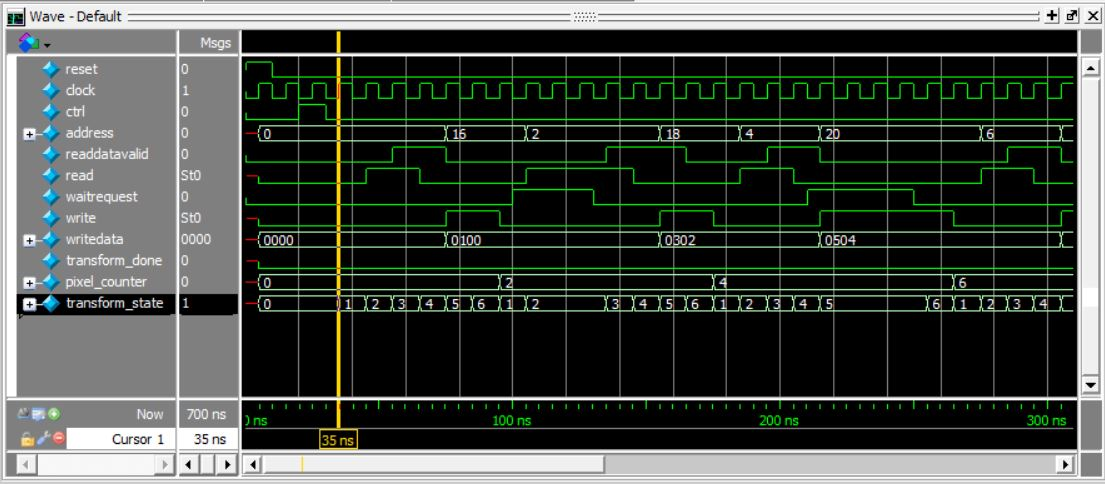
\includegraphics[width=0.8\textwidth]{figures/sim0.JPG}
        \caption{copy image without transformation}
        \label{fig:sim0}
    \end{figure}

    Figure~\ref{fig:sim1} and \ref{fig:sim2} are simulation results for rotation and flipping.
        \begin{figure}[h]
        \centering
        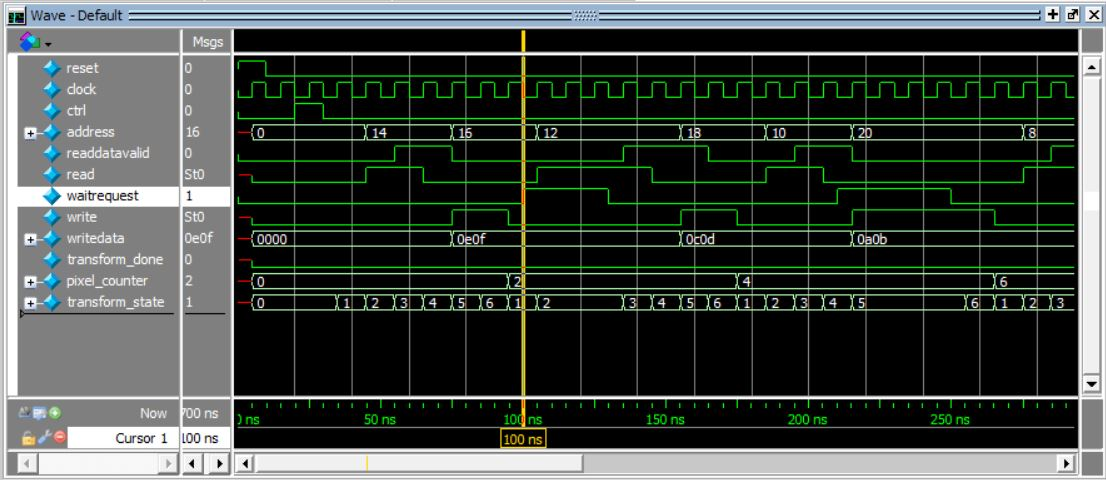
\includegraphics[width=0.8\textwidth]{figures/sim1.JPG}
        \caption{copy image with rotation by $180^\circ$}
        \label{fig:sim1}
    \end{figure}
    
        \begin{figure}[h]
        \centering
        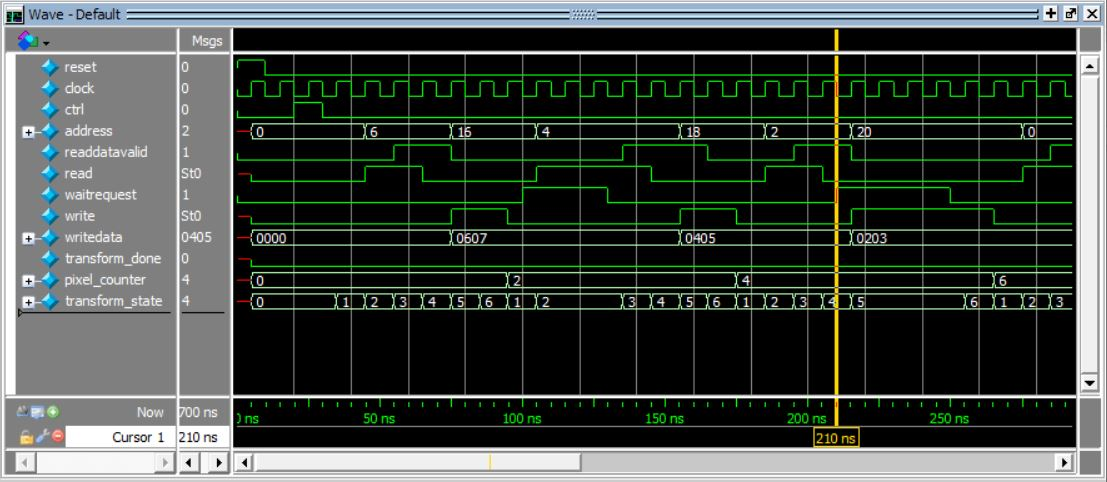
\includegraphics[width=0.8\textwidth]{figures/sim2.JPG}
        \caption{copy image with horizontal flip}
        \label{fig:sim2}
    \end{figure}
\end{enumerate}


\newpage
\section*{Part II}
In this part of the exercise we will augment the application logic circuit from Part I to create an AFU that can be connected to a processor. This step requires using Platform Designer, as well as the use of hardware development tools that are provided on the DevCloud. For this exercise, we will use an Avalon Memory Mapped interface for the application logic circuit. \\
\\
As shown in Figure \ref{fig:dmaAFU}, the CCI-P to Avalon-MM Adapter converts the CCI-P interface to the Avalon-MM interface. A Memory Properties Factory(MPF) module is added between the MMIO Decoder Logic and the CCI-P to Avalon-MM Adapter. This module ensures that read responses from the DMA return in the order that they were issued, which is required by the Avalon-MM protocol.\\

\begin{figure}[h]
    \centering
    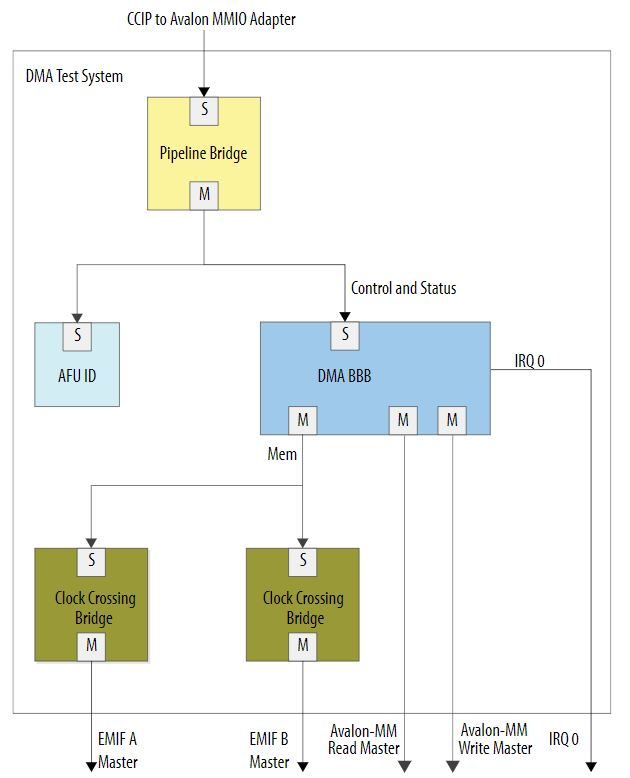
\includegraphics[width=0.5\textwidth]{figures/DMATestSystem.JPG}
    \caption{DMA Test System}
    \label{fig:dmaSystem}
\end{figure}

\noindent
Figure~\ref{fig:dmaSystem} illustrates the DMA Test System which provides the basic functionality of transfering data between the processor and local memory. The AFU ID component stores a 64-bit data pattern that is required for any AFU and also includes a {\it universally unique identifier}(UUID) for the AFU. The Pipeline Bridge connects the DMA BBB to the CCI-P to Avalon Adapter. The Clock Crossing Bridges connects the DMA BBB and the local FPGA SDRAM banks.\\ 
\\
Figure~\ref{fig:dmaBBB} gives a more detailed view of the DMA BBB subsystem. The main component is the Modular Scatter-Gather DMA (MSGDMA). It performs memory-mapped transfers between source and destination addresses in the host processor and the FPGA's memory. The data transferred by the MSGDMA must be aligned to 64-byte boundary. The Address Span Extender implements the memory transfer that are not aligned on 64-byte boundary. The Magic Number ROM component contains a single, read-only 64-byte value, which is used to create a write fence in host memory. The BBB ID component stores the UUID for the DMA BBB. It will be scanned by a software driver to identify the functionality of this DMA BBB.\\

\begin{figure}[h]
    \centering
    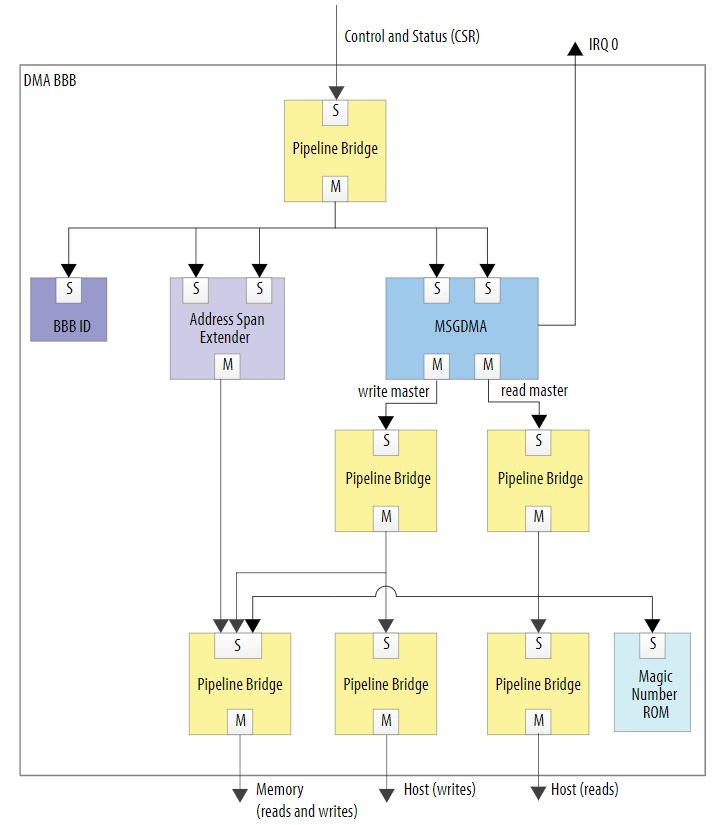
\includegraphics[width=0.5\textwidth]{figures/DMABBB.JPG}
    \caption{DMA BBB}
    \label{fig:dmaBBB}
\end{figure}

\noindent
We will integrate the module created in Part I into the DMA Test System to add the functionality of image transformation. In order for the processor to access the registers in {\it image\_transform} module, the module needs to be connected to the MMIO channel through the Pipeline Bridge. Meanwhile, the module needs to be connected to the Clock Crossing Bridges, which is connected with the local memory.\\
\\
Since the IPs inside the DMA Test System connects through the Avalon-MM interface, the {\it image\_transform} module needs to have an Avalon-MM slave interface to interact with the Pipeline Bridge and an Avalon-MM master interface to interact with the Clock Crossing Bridges. We name the slave interface {\it s0} and the master interface {\it m0}.\\
\\
The {\it s0} interface has ports {\it s0\_write}, {\it s0\_writedata} and {\it s0\_address}, which are corresponding to the {\it ctrl}, {\it ctrl\_data} and {\it ctrl\_address} input ports in Part I. The interface also has a 1-bit input {\it s0\_read} and 64-bit output {\it s0\_readdata}, which is used for the processor to get the status of an image transformation. When {\it s0\_read} is 1 AND {\it s0\_address} is 1, the component need to set {\it s0\_readdata} to the value of the {\it transfer\_done} register.\\
\\
\newpage
The {\it m0} interface has four output ports {\it address}, {\it writedata}, {\it read} and {\it write}, and three input ports {\it readdata}, {\it readdatavalid} and {\it waitrequest} which have the same functionality as in Part I. \\
\\

\begin{figure}[h]
    \centering
    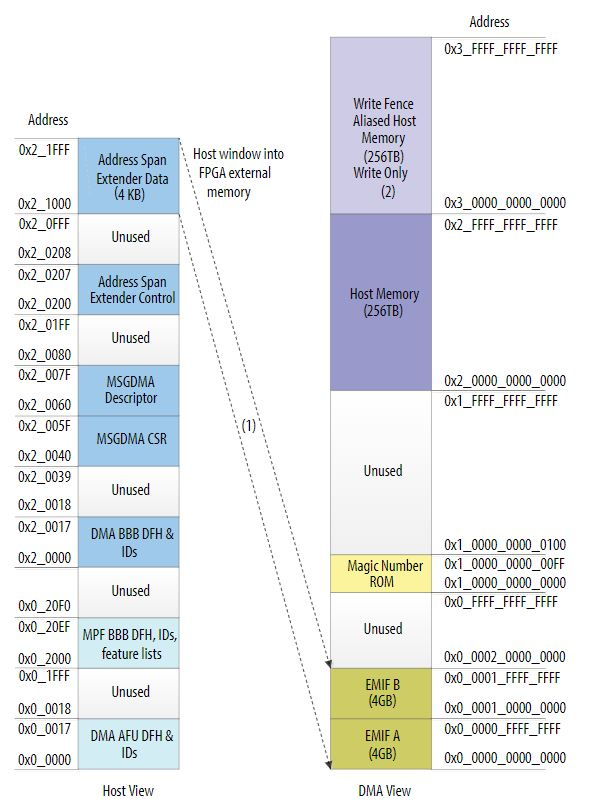
\includegraphics[width=0.5\textwidth]{figures/memoryView.JPG}
    \caption{the DMA AFU and host views of memory}
    \label{fig:memView}
\end{figure}

\noindent
In addition, we need to specify an address for the host to access registers in the image transformation component and also the address for the image transformation component to access the FPGA's local memory. Figure~\ref{fig:memView} shows the host view and the DMA AFU's view of the address space in the sample design. In the host view, the address space for the DMA system spans from 0x0\_0000 to 0x2\_1FFF. We can choose an unused block of addresses as the addresses for the image transformation component's registers. In the DMA view, the lowest two blocks of memory map to the two banks of local DDR SDRAM. Thus, the image transformation component accesses image data from address 0x0 to 0xFFFF\_FFFFF.\\
\\


\noindent
Perform the following steps to integrate the image transformation module into this DMA system:

\begin{enumerate}
    \item Finish the Verilog code for the image transformation module. Figure \ref{fig:templatePart2} shows a template for the image transformation module with the Avalon interfaces. Note that this code is very similar to that from Figure \ref{fig:templatePart1}. You can make the same assumption as in Part II that the original image starts at address 0, and the result image starts at address $total\_number\_of\_pixels$. You can also assume that the original image to flip horizontally has a multiple of $n/8=64$ pixels in each row. 
    \item Create a new project called \emph{dma\_test\_system} in Quartus. Ensure you are using the same version of Quartus as exists on the DevCloud (19.2 most recently). Proper functionality is not guaranteed with a different version. Select Arria 10 as the device family and use the default device. Copy all the files in \texttt{hw/rtl/qsys/A10} in \emph{design\_files} included along with this exercise 
    to the folder for your new project. Set \texttt{dma\_test\_system.qsys} as the top-level design.
    \item Create a new IP component called \emph{image\_transform} with the Verilog file using the Component Editor in Platform Designer.
    \begin{itemize}
        \item In tab \texttt{Component Type}, set the component name to \emph{image\_transform}.
        \item In tab \texttt{Files}, add your \texttt{image\_transform.sv} to \texttt{Synthesis Files}. Click \texttt{Analyze HDL Files}. If the analysis failed, fix the errors and re-analyze the file.
        \item In tab \texttt{Signals \& Interfaces}, set the interface names and types and signal types and direction as in Figure \ref{fig:ip_port}. 
        \item Set the \texttt{Associated Clock} for $m0$ and $s0$ to $clock$ and \texttt{Associated Reset} to $reset$. There should be no error in \texttt{Messages}.
        \item Click \texttt{Finish} button to create the IP component. Click \texttt{Yes,save} to save the \emph{image\_transform\_hw.tcl} file.
        \item Create a subfolder \texttt{image\_transform} in your project folder. Put \emph{image\_transform.sv} and \emph{image\_transform\_hw.tcl} into the subfolder. Depending on where the tcl file is created, you may need to change the \texttt{SYSTEM\_VERILOG PATH} in Line \emph{add\_filelist\_file} to \emph{image\_transform.sv}:
        \begin{lstlisting}
        add_fileset_file image_transform.sv SYSTEM_VERILOG PATH [original path] TOP_LEVEL_FILE
        \end{lstlisting}
    \end{itemize}
    \begin{figure}[h]
        \centering
        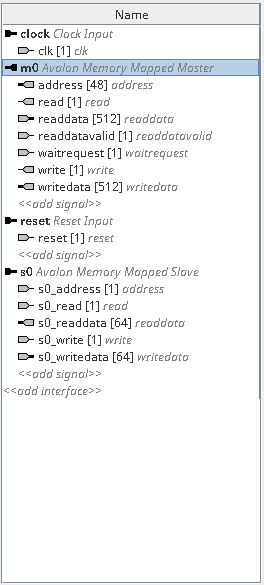
\includegraphics[width=0.25\textwidth]{figures/ip_port.JPG}
        \caption{IP Signals \& Interfaces}
        \label{fig:ip_port}
    \end{figure}
    \item Create an instance of image\_transform in the DMA system (\emph{dma\_test\_system.qsys}), setting the parameter \emph{n} to 512 and \emph{NUM\_BYTES} to \emph{n/8=64}. Make the following connections:
        \begin{itemize}
            \item connect clock to host\_clk.out\_clk
            \item connect reset to reset\_in.out\_reset
            \item connect s0 to dma\_test\_system\_mm\_bridge\_0.m0
            \item connect m0 to ddr4\_mm\_bridge.s0
        \end{itemize}
        The resulting connections are shown in Figure \ref{fig:ip_connect}.
        \begin{figure}
            \centering
            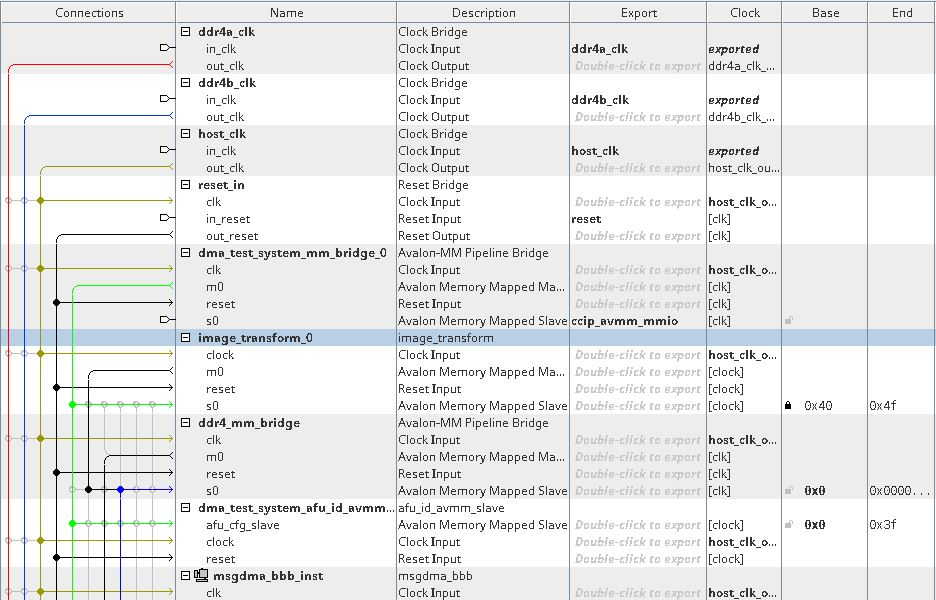
\includegraphics[width=0.9\textwidth]{figures/ip_connection.JPG}
            \caption{Connect IP interface}
            \label{fig:ip_connect}
        \end{figure}
    \item Set the base address of s0 of image\_transform to 0x0040, which is the first address available after the address space of the AFU ID component. 
    \item Save the qsys files for the DMA system.
\end{enumerate}

~\\
\noindent
Perform the following steps to complete the design of the AFU:

\begin{enumerate}
\item
Make a new folder on your home computer called \texttt{dma\_afu}. Then, in this folder create two subfolders named \texttt{hw} and \texttt{sw}. The \texttt{sw} folder will be used in Part 3 and 4 of this exercise. Now, in the \texttt{hw} folder make a subfolder called \texttt{rtl}. This arrangement of folders is required when using the compilation tools that are provided on the DevCloud.
\item
In your \texttt{rtl} subfolder, create a subfolder called \texttt{qsys}, and within that a subfolder called \texttt{A10}. Copy all the design files in your \emph{dma\_test\_system} project to the \texttt{A10} folder. \\
\\
Besides the DMA system, some other files are also provided in \texttt{design\_files/hw/rtl}. Copy the top-level file \emph{afu.sv} to your \texttt{rtl} folder. You also need to copy \emph{ccip\_interface\_reg.sv}, \emph{ccip\_std\_afu.sv} and the files in \texttt{BBB\_cci\_mpf} and \texttt{BBB\_ccip\_avmm} folders. These files specify the CCI-P interface and convert it to the Avalon Memory Mapped interface for the DMA system.\\
\\
The development tools on the DevCloud also requires \emph{filelist.txt}, which provides the path to all the design files for the DMA AFU, and \emph{dma\_afu.json}, which gives some important information about the AFU. Copy the two files into the \texttt{rtl} folder.

\item
Since we add the \emph{image\_transform} IP to the DMA AFU, we need to include the paths to the design files (\emph{.sv} and \emph{.ip} file) of this IP core in \emph{filelist.txt}. The paths are relative to the directory containing \emph{filelist.txt}:
\begin{lstlisting}
qsys/A10/image_trasform/image_transform.sv
qsys/A10/ip/dma_test_system/dma_test_system_image_transform_0.ip
\end{lstlisting}

\item
For the remainder of this exercise we assume that you are able to login to the DevCloud and configure the environment variables and settings that are needed for AFU development.  First, copy the folder \texttt{dma\_afu} and its subfolders onto the DevCloud.  Then, 
using the Linux command line interface on the DevCloud execute the command 
\texttt{uuidgen} to generate a new UUID for the DMA AFU.
Enter this new UUID into the file {\it hw/rtl/dma\_afu.json}, replacing the value of the key \emph{accelerator-type-uuid}.\\
\\
Update the parameter \emph{AFU\_ID\_H}  and \emph{AFU\_ID\_L} of \emph{dma\_test\_system\_afu\_id\_avmm\_slave\_0.ip} to the upper 16 digits and lower 16 digits of the new UUID. You must enter this in decimal, and you may use a calculator to make the conversion. For example, the UUID "633b3709-4b4a-415e-bddc-fd2e07e8d5e8" should be entered as: \emph{AFU\_ID\_H} = 7150369346438185310 and \emph{AFU\_ID\_L} = 13681088142187746792. The IP file is in \texttt{hw/rtl/qsys/A10/ip/dma\_test\_system/}.

\item
On the DevCloud, set your working directory to the \texttt{dma\_afu} folder, and then 
run the command: 

\noindent
\texttt{afu\_synth\_setup -s hw/rtl/filelist.txt build\_synth}

Now, change your working directory to the newly-created \texttt{build\_synth} folder and 
execute the command \texttt{run.sh}. 
The \texttt{run.sh} command then executes the Intel 
Quartus\textsuperscript{\textregistered} Prime software to compile the AFU into a circuit
that can be implemented in the target FPGA device.

~\\
\noindent
The Quartus Prime software begins by executing its synthesis tools that
compile your Verilog source code. If any syntax errors are reported (they are shown in 
\red{red}), then fix these errors and compile again. Note that it is 
``normal'' to receive a significant number of warning messages from the Quartus Prime 
software when compiling an AFU; while you should still monitor these messages, those that
refer to code that is not part of your \emph{image\_transform} IP file can usually be ignored.

~\\
\noindent
After successful compilation of your AFU code, the Quartus Prime software generates an FPGA 
programming bit-stream file called {\it dma\_afu.gbs}. You can download this {\it gbs} file into the FPGA device on the DevCloud by executing the command:

\noindent
\texttt{fpgasupdate dma\_afu.gbs}.

Note that if you are using version 1.2.1 of the Arria 10 Development Stack on the
DevCloud, then you have to execute two commands to program the FPGA. First, execute:

\noindent
\texttt{PACSign PR -t UPDATE -H openssl\_manager -i dma\_afu.gbs -o dma\_afu\_unsigned.gbs}

\noindent Type \texttt{y} ({\it yes}) in answer to the queries that are issued by this command. 
Then, execute:

\noindent
\texttt{fpgasupdate dma\_afu\_unsigned.gbs}.
\end{enumerate}
~\\
\noindent
Now that the AFU has been downloaded into the target FPGA device, we can develop software 
programs which run on the processor and make use of the AFU.

\lstset{language=Verilog,morekeywords={logic,always_ff},numbers=none,escapechar=|}
\begin{figure}[h]
\begin{center}
\begin{minipage}[h]{15 cm}
\begin{lstlisting}[name=code]
module image_transform(clk, reset, s0_write, s0_writedata, s0_address, s0_read, s0_readdata, readdata, readdatavalid, waitrequest, address, read, write, writedata);
    parameter NUM_BYTES = 64, n = 512;

    input clk, reset, s0_write, s0_read, s0_address;
    input [63:0] s0_writedata;
    output logic [63:0] s0_readdata;

    input [n-1:0] readdata;
    input readdatavalid, waitrequest;
    output logic [47:0] address;
    output logic read, write;
    output logic [n-1:0] writedata;

    logic transform_done;
    logic [31:0] pixel_counter;
    logic [15:0] pixel_per_row;
    logic [47:0] src_address, dst_address;
    logic [ 7:0] transform_type;
    // ... declare other signals

    wire ctrl, ctrl_address;
    wire [63:0] ctrl_data;
    assign ctrl = s0_write;
    assign ctrl_data = s0_writedata;
    assign ctrl_address = s0_address;

    always @(posedge clk) begin
        if(reset)
            s0_readdata <= '0;
        else if(s0_read && s0_address == 1)
            s0_readdata[0] <= transform_done;
    end

    always @(posedge clk) begin
        if(reset) begin
            src_address <= '0; dst_address <= '0; 
            transform_type <= '0;
        end
        else if(ctrl && ctrl_address == 0) begin    // read instructions
            src_address <= '0;
            dst_address[31:0] <= ctrl_data[63:32];
            pixel_per_row   <= ctrl_data[31:16];
            transform_type  <= ctrl_data[7:0];
        end
    end

    // ... define transform_done
    // ... define finite state machine
endmodule

\end{lstlisting}
\end{minipage}
\caption{A template for the image transform Verilog code.}
\label{fig:templatePart2}
\end{center}
\end{figure}

\section*{Part III}
An example of a C program that uses the OPAE infrastructure to perform direct memory access is given in Figure \ref{fig:C_code}. This code includes the header file {\it fpga\_dma.h} which defines the API for setting up communication with the DMA BBB in the AFU and controlling the DMA BBB for data transfers. \\

\lstset{language=C,numbers=left,escapechar=\^}
\begin{figure}
\begin{center}
\begin{minipage}[h]{17 cm}
\begin{lstlisting}[name=C_code]
int main(int argc, char *argv[]){
	if (argc < 2) {
		printf("Usage: fpga_dma_test <path to image>\n");
		return -1;
	}
	
	fpga_result res = FPGA_OK;
	fpga_dma_handle dma_h;
	fpga_handle afc_h;
	uint64_t *dma_buf_ptr = NULL;

	^\label{line:dma_open}^if(open_AFU(&afc_h) < 0)
		return -1;
	res = fpgaDmaOpen(afc_h, &dma_h);
	if(res != FPGA_OK || !dma_h)
		return -1;

	unsigned char * data, header;
	int width, height;
	if (read_grayscale(argv[1], &header, &data, &width, &height) < 0) 
		return -1;
	
	uint64_t count = width * height;
	^\label{line:dma_buf}^dma_buf_ptr = (uint64_t *)malloc_aligned(getpagesize(), count);
	if (!dma_buf_ptr)
		return -1;
	fill_buffer((char *)dma_buf_ptr, data, count);

	// copy from host to fpga
	^\label{line:dma_htom}^res = fpgaDmaTransferSync(dma_h, 0x0 /*dst */,
				  (uint64_t)dma_buf_ptr /*src */, count, HOST_TO_FPGA_MM);
	if(res != FPGA_OK)
		return -1;
	clear_buffer((char *)dma_buf_ptr, count);
	
	// copy from fpga to fpga
	^\label{line:dma_fpga}^res = fpgaDmaTransferSync(dma_h, count /*dst */, 
	               0x0 /*src */, count, FPGA_TO_FPGA_MM);
	if(res != FPGA_OK)
		return -1;

	// copy from fpga to host
	^\label{line:dma_mtoh}^res = fpgaDmaTransferSync(dma_h, (uint64_t)dma_buf_ptr /*dst */,
				  count /*src */, count, FPGA_TO_HOST_MM);
	if(res != FPGA_OK)
		return -1;

	write_result((char *)dma_buf_ptr, header, width, height);

	if (dma_buf_ptr)
		free_aligned(dma_buf_ptr);
	if (dma_h)
		res = fpgaDmaClose(dma_h);

	close_AFU(afc_h);
	return 0;
}
\end{lstlisting}
\end{minipage}
\caption{Using the AFU in a C program (a)}
\label{fig:C_code}
\end{center}
\end{figure}


\lstset{language=C,numbers=left,escapechar=|}
\begin{figure}
\begin{center}
\begin{minipage}[h]{17 cm}
\begin{lstlisting}[name=C_code]
static inline void fill_buffer(char *buf, unsigned char *data, size_t size){
    memcpy(buf, data, size);
}

static void write_result(char *buf, unsigned char *header, int width, int height){
	write_grayscale_bmp("result.bmp", header, (unsigned char *)buf, width, height);
}

static inline void clear_buffer(char *buf, size_t size){
	memset(buf, 0, size);
}
\end{lstlisting}
\end{minipage}
\caption{Using the AFU in a C program (b)}
\label{fig:C_code}
\end{center}
\end{figure}

\noindent
In Line \ref{line:dma_open}, the \emph{fpgaDMAOpen} function sets up additional environment for the direct memory access. The function first searches for the DFH of the DMA BBB in the opened AFU. If the DMA BBB is in the AFU, the function calls \emph{fpgaPrepareBuffer} to allocate page-aligned memory for shared access between the AFU and the software program. Then, it initializes a handle \emph{dma\_h} to the DMA BBB. If all steps are done successfully, it returns \texttt{FPGA\_OK}, otherwise it returns an error code. \\
 \\
\newpage
The code then reads an image and creates a buffer to store it. Note that the allocated buffer needs to be at a page-size aligned address because it will be mapped to the shared memory buffers during data transfers, which are required to be page-aligned.\\
\\
% The remainder of the code uses DMA via the \emph{dma\_h} variable to access the registers in the DMA BBB. The \emph{fpgaDMATransferSync} function performs a transfer between a source address and a destination address. It controls the MSGDMA's descriptor to let the AFU move data inside the FPGA's local memory or between the FPGA's local memory and the shared memory. If doing a host to FPGA or FPGA to host transfer, it will create a copy of data between source/destination address and the shared memory. This function is a blocking call and returns when the transfer completes.\\
% \\
\noindent
The  remainder of the code transfers an image between a source address and a destination address by calling the function \emph{fpgaDMATransferSync}. It controls the components in the DMA BBB in Figure \ref{fig:dmaBBB} via the \emph{dma\_h} variable to move data between the FPGA's local memory and the shared memory. The pointer to the buffer allocated in Line \ref{line:dma_buf} is used as the \emph{src} address for the host-to-FPGA transfer (Line \ref{line:dma_htom}) and also the \emph{dst} address for the FPGA-to-host transfer (Line \ref{line:dma_mtoh}). The \emph{dst} address of the host-to-FPGA transfer is set to 0x0 and the \emph{src} address of the FPGA-to-host transfer is set to the size of image (\emph{count}), which are addresses in the FPGA's local memory in the DMA View. The FPGA-to-FPGA transfer (Line \ref{line:dma_fpga}) transfers the image from 0x0 to \emph{count}. The \emph{fpgaDMATransferSync} function is a blocking call and returns a \emph{fpga\_result} when the transfer completes. \\
\\
To complete this part of the exercise perform the following steps:
\begin{enumerate}
    \item Copy the files in the \texttt{design\_files/sw} that accompany this exercise to the \texttt{sw} folder for the AFU on the DevCloud. The file \emph{part3.c} contains the code shown in Figure \ref{fig:C_code}. \emph{image\_helper.c} provides helper functions to read and write BMP images. \emph{manage\_afu.c} holds the code for \emph{open\_AFU} and \emph{close\_AFU}. The header file \emph{fpga\_dma.h} define the API for using a DMA AFU. The files \emph{fpga\_dma.c} and \emph{fpga\_dma\_internal.h} provides an implementation for the API functions.
    \item In the \texttt{sw} directory on the DevCloud run the command \verb|make part3|. To execute your program type \verb| ./part3 [path to source image] |.
    \item An image \emph{result.bmp} will be created when the program finishes. 
\end{enumerate}


\section*{Part IV}
For this part of the exercise you are to write a C program to do image transformation using the AFU. The OPAE header file {\it mmio.h} includes functions for accessing control registers through memory-mapped I/O. You can make use of the functions {\it fpgaWriteMMIO64} and {\it fpgaReadMMIO64} to send the start command and get the status of a transformation.  To transfer the source image and the result image, you can use the {\it fpgaDMATransferSync} function from {\it fpga\_dma.h}. \\
\\
Perform the following:
\begin{enumerate}
    \item Write your C code in a file {\it part4.c}. The code should write to the {\it image\_transform} component at address $0x40$, which is the base address we choose for {\it s0} of the {\it image\_transform} IP as shown in Figure \ref{fig:ip_connect}, and read from address $0x48$, which corresponds to the address offset 1 in the {\it image\_transform} IP.\\
    \\
    Notice that in Part II, we assume that the image to flip horizontally has a multiple of 64 pixels in each row. You may need to pad an image to satisfy this requirement. Your program should take two arguments, one for the path to the image to process, the other for the type of image transformation the AFU to perform (0: no transformation, 1: rotating by $180^\circ$, 2: horizontal flip). 
    
    \item To compile your code on the DevCloud, put {\it part4.c} into your {\it sw} folder and execute \verb|make part4|. Run \verb|./part4 [path to image] [transformation type]| to run the program.
\end{enumerate}

%%%%%%%%%%%%%%%%%%%%%%%%%%%%%%%%%%%%%%%%
%%% FPGAcademy Copyright Information %%%
%%%%%%%%%%%%%%%%%%%%%%%%%%%%%%%%%%%%%%%%

%Always put the copyright on a new page (clear page), with some vertical space from top
\clearpage
\vspace{1in}

\noindent

Copyright {\copyright} FPGAcademy.org. All rights reserved. FPGAcademy and the 
FPGAcademy logo are trademarks of FPGAcademy.org.  This document is provided 
"as is", without warranty of any kind, express or implied, including but not 
limited to the warranties of merchantability, fitness for a particular purpose 
and noninfringement. In no event shall the authors or copyright holders be 
liable for any claim, damages or other liability, whether in an action of 
contract, tort or otherwise, arising from, out of or in connection with the 
document or the use or other dealings in the document.
~\\
~\\
**Other names and brands may be claimed as the property of others.



\end{document}
